\begin{frame}{Kyllingestriber}

\small

\begin{columns}[T]

\begin{column}{0.58\textwidth}

\textbf{Regler for kyllingestriber:}

\begin{itemize}[]
\item Tilsås med 30\% udsædsmængde (synlig reduktion ift. tilstødende areal)
\item Minimum 3 m brede
\item Skal kombineres med tiltaget "sprøjte- og gødningsfri randzone"
\end{itemize}

\vspace{0.4em}

\textbf{Gavner arter:}

\footnotesize
Agerhøne, fasan, sanglærke, vibe, markpiber, gul vipstjert, 
rødrygget tornskade, gulspurv, agerpistol, vilde bier, humlebier, 
dagsommerfugle, rovbiller, græshopper, markmus, pindsvin, musvåge, tårnfalk

\end{column}

\begin{column}{0.40\textwidth}
\centering
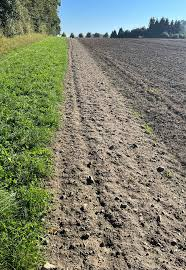
\includegraphics[width=\textwidth]{Billeder/Vildtforvaltning/biotopplantiltag/kyllingestriber.jpeg}
\end{column}

\end{columns}

\end{frame}